\documentclass[border=3pt,tikz]{standalone}
\usepackage[utf8]{vietnam}
\usetikzlibrary{calc,angles,intersections,shapes.geometric,arrows,decorations.markings,arrows.meta,patterns.meta,patterns}
\usepackage{tikz-3dplot,pgfplots}
\pgfplotsset{compat=1.15}
\usepgfplotslibrary{polar}
\usepackage{amsmath}
\tikzset{My Line Style/.style={ultra thick, blue, fill=yellow!10, fill opacity=0.5,join=round}}
\begin{document}
	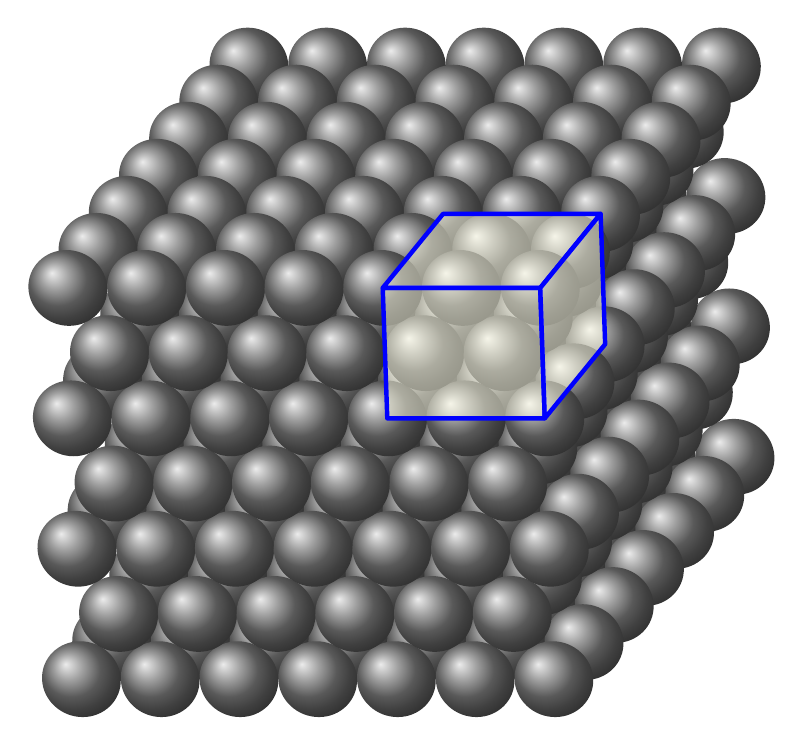
\begin{tikzpicture}[rotate around x=5] 
		\foreach \x in {0,1,2,3,4,5,6}{% 
			\foreach \z in {0,1,2,3,4,5,6}{%      
				\shade[ball color=gray] (\x,0,\z) circle(0.5);
			}
		}
		\foreach \x in {0.5,1.5,2.5,3.5,4.5,5.5}{%
			\foreach \z in {0,1,2,3,4,5,6}{%
				\shade[ball color=gray] (\x,{sqrt(0.74)},\z) circle(0.5);
			}
		}
		\foreach \x in {0,1,2,3,4,5,6}{%
			\foreach \z in {0,1,2,3,4,5,6}{%
				\shade[ball color=gray] (\x,{2*sqrt(0.74)},\z) circle(0.5);
			}
		}
		\foreach \x in {0.5,1.5,2.5,3.5,4.5,5.5}{%
			\foreach \z in {0,1,2,3,4,5,6}{%
				\shade[ball color=gray] (\x,{3*sqrt(0.74)},\z) circle(0.5);
			}
		}
		\foreach \x in {0,1,2,3,4,5,6}{%
			\foreach \z in {0,1,2,3,4,5,6}{%
				\shade[ball color=gray] (\x,{4*sqrt(0.74)},\z) circle(0.5);
			}
		}
		\foreach \x in {0.5,1.5,2.5,3.5,4.5,5.5}{%
			\foreach \z in {0,1,2,3,4,5,6}{%
				\shade[ball color=gray] (\x,{5*sqrt(0.74)},\z) circle(0.5);
			}
		}
		\foreach \x in {0,1,2,3,4,5,6}{%
			\foreach \z in {0,1,2,3,4,5,6}{%
				\shade[ball color=gray] (\x,{6*sqrt(0.74)},\z) circle(0.5);
			}
		}
		
		\draw [My Line Style] (6,{4*sqrt(0.74)},6) -- (4,{4*sqrt(0.74)},6) -- (4,{6*sqrt(0.74)},6) -- 
		(6,{6*sqrt(0.74)},6) -- cycle;
		\draw [My Line Style] (4,{6*sqrt(0.74)},6) -- (4,{6*sqrt(0.74)},4) -- (6,{6*sqrt(0.74)},4) --
		(6,{6*sqrt(0.74)},6) -- cycle;
		\draw [My Line Style] (6,{4*sqrt(0.74)},6) -- (6,{4*sqrt(0.74)},4) -- (6,{6*sqrt(0.74)},4) --
		(6,{6*sqrt(0.74)},6) -- cycle;
	\end{tikzpicture}
\end{document}